\documentclass[11pt]{article}
\usepackage{report}

\usepackage[utf8]{inputenc} % allow utf-8 input
\usepackage[T1]{fontenc}    % use 8-bit T1 fonts
\usepackage[colorlinks=true, linkcolor=black, citecolor=blue, urlcolor=blue]{hyperref}       % hyperlinks
\usepackage{url}            % simple URL typesetting
\usepackage{booktabs}       % professional-quality tables
\usepackage{amsfonts}       % blackboard math symbols
\usepackage{nicefrac}       % compact symbols for 1/2, etc.
\usepackage{microtype}      % microtypography
\usepackage{lipsum}		% Can be removed after putting your text content
\usepackage{graphicx}
\graphicspath{ {./images/} }
\usepackage{natbib}
\usepackage{doi}
\setcitestyle{aysep={,}}
\usepackage{array}
\usepackage{listings}

\usepackage{xcolor}
\definecolor{codegreen}{rgb}{0,0.6,0}
\definecolor{codegray}{rgb}{0.5,0.5,0.5}
\definecolor{codeorange}{rgb}{1,0.49,0}
\definecolor{backcolour}{rgb}{0.95,0.95,0.96}

\lstdefinestyle{mystyle}{
    backgroundcolor=\color{backcolour},   
    commentstyle=\color{codegray},
    keywordstyle=\color{codeorange},
    numberstyle=\tiny\color{codegray},
    stringstyle=\color{codegreen},
    basicstyle=\ttfamily\footnotesize,
    breakatwhitespace=false,         
    breaklines=true,                 
    captionpos=b,                    
    keepspaces=true,                 
    numbers=left,                    
    numbersep=5pt,                  
    showspaces=false,                
    showstringspaces=false,
    showtabs=false,                  
    tabsize=2,
    xleftmargin=10pt,
}

\lstset{style=mystyle}
\title{CT248 - Introduction to Modelling}

\author{Andrew Hayes\\
\AND
Student ID: 21321503\\
\AND
\AND
\AND
\AND
	1BCT1\\
\AND
	NUI Galway\\
}

% Uncomment to remove the date
\date{February 2022}

% Uncomment to override  the `A preprint' in the header
\renewcommand{\headeright}{Introduction to Modelling}
\renewcommand{\undertitle}{Introduction to Modelling}
\renewcommand{\shorttitle}{}

%%% Add PDF metadata to help others organize their library
%%% Once the PDF is generated, you can check the metadata with
%%% $ pdfinfo template.pdf
% \hypersetup{
% pdftitle={A template for the arxiv style},
% pdfsubject={q-bio.NC, q-bio.QM},
% pdfauthor={David S.~Hippocampus, Elias D.~Striatum},
% pdfkeywords={First keyword, Second keyword, More},
% }

\begin{document}
\maketitle

\newpage
\tableofcontents
\thispagestyle{empty}


\newpage
\setcounter{page}{1}
\section{Lecture 01 - MATLAB Overview}
\textbf{MATLAB} (MAtrix LABoratory) is a powerful technical computing system for handling scientific \& engineering 
calculations, designed to make \textbf{matrix computations} particularly easy. 
It is a \textbf{high-level language} with an interactive development environment.
MATLAB is \textbf{loosely typed}.

MATLAB is used for:
\begin{itemize}
    \item Numerical computation. 
    \item Data analysis \& visualisation. 
    \item Algorithm development \& programming. 
    \item Application development \& deployment.
\end{itemize}

\subsection{Variables}
A variable name in MATLAB may consist only of letters a-z, digits 0-9, and the underscore (\_) and they must start
with a letter. 
A variable name may not exceed 63 characters. 
MATLAB is case-sensitive, including command \& function names. 

The use of a semi-colon \verb|;| at the end of a variable initialisation prevents the value from being displayed. 

\verb|carSpeed = 20;|

\subsubsubsection{The MATLAB Workspace}
All variables created during a session remain in the workspace until they are \textbf{cleared}. 
\begin{lstlisting}[language=MATLAB]
clear;
mph = input("Please enter the speed in mph: ");
kph = mph * 1.6;
fprintf("%d mph = %d kph\n",mph,kph);
\end{lstlisting}

The command \verb|who| lists all the names in the current workspace. 
The command \verb|whos| lists the size of each variable. 

Comments can be made in MATLAB using the \verb|%| sign. 

\subsection{Expressions}
An \textbf{expression} is a formula consisting of variables, numbers, operators, \& function names. 
Expressions are evaluated when you enter them into the MATLAB prompt. 
Note that MATLAB uses the function \verb|ans| to return the last expression that was evaluated but not assigned
to a variable. 

\subsubsection{Statements}
MATLAB \textbf{statements} are frequently of the form \verb|variable = expression|. \\
E.g.: \verb|s=u*t-g/2*t.^2|. 
\\
This is an example of an \textbf{assignment statement}, with the value of the expression assigned to the 
variable on the left-hand side.
A semicolon is at the end to suppress the output. 

Statements that are too long for a line can be extended to several lines with an ellipsis of at least 3 dots \verb|...|
\\
Statements on the same line can be separated by commas or semicolons.

\newpage

\subsection{Input \& Output}
The \verb|input()| statement is used to read in input data. 
\begin{lstlisting}[language=MATLAB]
name = input ("Enter your name: ");
\end{lstlisting}

The \verb|disp()| statement is used to \textbf{display} data. 
The general form of the \verb|disp| statement is \verb|disp(variable)|. 

\begin{lstlisting}[language=MATLAB]
>> disp("Hello World!")
>> x = 2;
>> disp(["The answer is ", num2str(x)])
The answer is 2. 
>> disp([2 3 x])
2.00 3.00 2.00
\end{lstlisting}

To display more than one variable, embed the variables into an \textbf{array}. 
All components of a MATLAB array must be the same type.

\begin{lstlisting}[language=MATLAB]
% Script file for converting temperatures from F to C. 
% Step 1: Get the input
F = input ("Enter the temperature in degrees F: ");

% Step 2: Convert to C 
 C = (F -32) * 5/9;

% Step 3: Display the result
fprintf("The temperature of %f (F) is %f (C)\n",F,C);
\end{lstlisting}

\subsection{Arithmetic Operators}
The evaluation of an expression is achieved by means of arithmetic operators. 
The arithmetic operations on two scalar constants / variables is shown. 
Left division may seem curious, however \textit{matrix} left division has an entirely different meaning. 

\begin{center}
\begin{tabular}{ |c|c|c| } 
    \hline
    \textbf{Operation} & \textbf{Algebraic Form} & \textbf{MATLAB} \\ 
    \hline
    Addition        & $ a + b $                 & \verb|a + b|  \\ 
    \hline
    Subtraction     & $ a - b $                 & \verb|a - b|  \\ 
    \hline
    Multiplication  & $ a \times b  $           & \verb|a*b|    \\
    \hline
    Right Division  & $ a/b $                   & \verb|a/b|    \\
    \hline
    Left Division   & $ b \textbackslash a $    & \verb|b\a|    \\
    \hline
    Exponent        & $ a^b $                   & \verb|a^b|    \\
    \hline
\end{tabular}
\end{center}

MATLAB uses PEMDAS as to determine \textbf{precedence}. 

\subsection{Repetition \& Loops - The For Loop}
The \verb|for| statement repeats some statement a specific number of times. 
The two basic \verb|for| loop structures are as follows:
\begin{lstlisting}[language=MATLAB]
for index = j:k 
    statements;
end 

for index = j:m:k 
    statements;
end
\end{lstlisting}

\verb|j:k| is a \textit{vector} with elements $j, j+1, j+2, \cdots, k$. 
\verb|j:m:k| is a vector with elements $j, j+m, j+2m, \cdots$ such that the final element does not exceed $k$. 
\verb|index| must be a variable. Loop statements should be indented.


\begin{lstlisting}[language=MATLAB]
for i = 1:5
    disp(i);
end
\end{lstlisting}

This for loop repeats the \verb|disp()| statement 5 times, starting with \verb|i = 1| and ending with \verb| i = 5|, incrementing by 1 each iteration of the loop. 

For a for loop of the form \verb|for i = a:b|, the number of iterations will be $b - a +1$.

The following example program takes in $n$ numbers and displays their average. 
\begin{lstlisting}
clear; 
sum = 0;

n = input("How many numbers: ");

for i=1:n 
    num = input("Please enter a number: ");
    sum += num;
end 

avg = sum/n; 

fprintf("The average is %f\n.", avg); 
\end{lstlisting}


\subsection{Relational Operators} 
\textbf{Relational Operators} form a logical expression that is either \textit{true} or \textit{false}.
Relational operators form the basis for decision logic. 

In MATLAB, "true" \& "false" can be represented both lexically (\verb|true|, \verb|false|) and logically (\verb|1|, \verb|0|). 
When returning the value of a Boolean expression or variable, MATLAB will use logical true (\verb|1|) \& false (\verb|0|). 

\begin{center}
    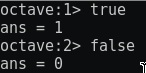
\includegraphics[width=0.25\textwidth]{truefalse.png}
\end{center}

\begin{center}
\begin{tabular}{ |c|c| } 
    \hline
    \textbf{Relational Operator} & \textbf{Meaning} \\ 
    \hline
    \verb|<|    & Less than                 \\ 
    \hline 
    \verb|<=|   & Less than or equal to     \\ 
    \hline 
    \verb|==|   & Equal to                  \\
    \hline 
    \verb|~=|   & Not equal to              \\ 
    \hline 
    \verb|>|    & Greater than              \\
    \hline 
    \verb|>=|   & Greater than or equal to  \\
    \hline
\end{tabular}
\end{center}

\subsubsection{The "If" Statement} 
In MATLAB, \verb|if| statements take the general form(s):
\begin{lstlisting}[language=MATLAB]
if condition; statements; end 

if condition
    statements
else
    statements
end

if condition
    statements
elseif condition
    statements 
else 
    statements
end
    
\end{lstlisting}

\begin{lstlisting}[language=MATLAB]
num = input("Enter a number: ");
if num < 0; disp("Negative number"); end
\end{lstlisting}

\section{Matrices}
In linear algebra, a \textbf{matrix} is a rectangular grid of numbers arranged into \textit{rows} \& \textit{columns}. 
An $r \times c$ matrix has $r$ rows \& $c$ columns. 
Uppercase letters (e.g., $A$) are usually used to denote variables that are matrices. 
$a_{ij}$ denotes the element in $A$ at row $i$ \& column $j$. 

\begin{center}
    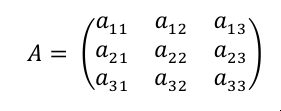
\includegraphics[width=0.25\textwidth]{matrix.png}
\end{center}

\subsection{Multiplying a Matrix by a Scalar}
A matrix $A$ can be multiplied by a scalar $k$, resulting in a matric of the same dimensions as $A$. 
The multiplication takes place in a straightforward fashion, with each element in the new matrix being the product of $k$ times the corresponding element in $A$. 

\begin{center}
    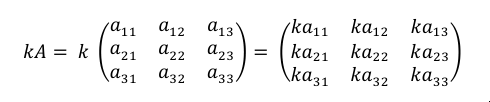
\includegraphics[width=0.5\textwidth]{matrixscalar.png}
\end{center}

Let matrix $C$ be the $r \times c$ product $AB$ of the $r \times n$ matrix $A$ with the $n \times c$ matrix B. 
Each element of $C$, $C_{ij}$, is equal to the vector dot product of row $i$ of $A$ with column $j$ of $B$. 

\begin{center}
    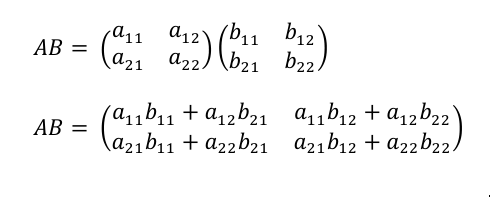
\includegraphics[width=0.5\textwidth]{2x2example.png}
\end{center}

In MATLAB, a matrix is a rectangular object consisting of rows \& columns. 
Matrices have comprehensive support with functions \& operators.
Rows can be separated when initialising a matrix using the semicolon \verb|;|. 

\begin{lstlisting}
>>a = [1 2 3; 4 5 6]
a = 
    1   2   3 
    4   5   6

>>a'
ans= 
        1   4 
        2   5 
        3   6
\end{lstlisting}


Individual elements are usually referenced with two subscripts in the form \verb|matrixname(row, column)|. 
However, elements can also be referenced using \textit{one} subscript. 
In this case, MATLAB will treat the entire vector as a single column.

\begin{lstlisting}[language=MATLAB]
A=[1 2 3;4 5 6;7 8 9] 
A(1,1)
A(1)
A(9)
\end{lstlisting}

Using the colon \verb|:| operator in place of a subscript denotes all the elements in the corresponding row or column. 
\verb|A(3,:)| means ``all the elements in the third row''. 
\verb|A(:,3)| means ``all the elements in the third column''. 
You can extract subsets of a matrix using something like \verb|A(1:2, 2:3)|.

\subsubsection{Matrix Functions}
\begin{center} \begin{tabular}{ |c|c| } 
    \hline
    \textbf{Function}   & \textbf{Description}                  \\ 
    \hline
    \verb|eye()|        & Identity Matrix                       \\
    \hline 
    \verb|linspace()|   & Vector with linearly spaced elements  \\
    \hline 
    \verb|ones()|       & Matrix of 1s                                      \\ 
    \hline 
    \verb|rand()|       & Uniformly distributed random numbers \& arrays    \\ 
    \hline 
    \verb|randn()|      & Normally distributed random numbers \& arrays     \\ 
    \hline 
    \verb|zeros()|      & Matrix of 0s.     \\ 
    \hline 
    \verb|det()|        & Determinant       \\ 
    \hline 
    \verb|eig()|        & Eigenvalues \& eigenvectors. \\
    \hline 
    \verb|expm()|       & Matrix exponential \\
    \hline 
    \verb|inv()|        & Matrix inverse    \\ 
    \hline 
    \verb|trace()|      & Sum of diagonal elements \\ 
    \hline 
    \verb|{}\| and \verb|/| & Linear equation solutions. \\
    \hline
\end{tabular}
\end{center}


\subsection{Vectors} 
A \textbf{vector} is a special type of matrix, having only one row or one column. 
MATLAB handles matrices \& vectors in the same way. 

Rules:
\begin{itemize}
    \item Elements in the list must be enclose in square brackets. 
    \item Elements in the list must be separated by either spaces or by commas. 
\end{itemize}

\begin{lstlisting}[language=MATLAB]
x = [1 2 3 4 5 6]
y = [1,2,3,4,5,6]
\end{lstlisting}

Vectors can also be initialised using the colon \verb|:| operator. 
\begin{lstlisting}[language=MATLAB]
x = 1:10 
y = 1:5:10
\end{lstlisting}

Operations can be performed on vectors, e.g \verb|sum(x)|, \verb|mean(x)|, etc. 
Elements in a vector can be accessed via \verb|x(1)| or \verb|x(1:3)| to get a range of elements. 
Note: vectors in MATLAB are indexed from 1, not 0. 

\subsubsection{Transposing Vectors} 
The vectors generated thus far have been \textit{row vectors}. 
\textit{Column vectors} may be needed for matrix operations. 
The single quote \verb|'| can be used to transpose a vector. 

\begin{center}
    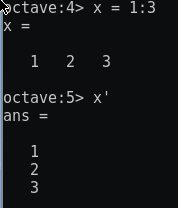
\includegraphics[width=0.25\textwidth]{singlequote.png}
\end{center}

\section{Lecture 02 - Logical Vectors \& Arrays}
\subsection{Element-Wise Operations}

\section{MATLAB Functions} 
MATLAB allows you to create your own function \textbf{M-files}. 
A function file differs from a script file in that the function M-file communicates with the MATLAB workspace through 
specially designated input \& output arguments. 

A function M-file \verb|name.m| has the following general form:
\begin{lstlisting}[language=MATLAB]
function [outarg1, outarg2, ...] = name(inarg1, inarg2, ...)
% help text
outarg1 = ...;
outarg2 = ...; 
end 
\end{lstlisting}

\begin{itemize}
    \item   \textbf{Function Keyword -} The function file must start with the keyword \verb|function|. 
    \item   \textbf{Input \& Output Arguments -} The input \& output arguments define the function's means of communication with the workspace. 
        \begin{itemize}
            \item   If there is more than one output argument, the output arguments must be separated by commas \& enclosed in square brackets. 
            \item   Input \& output variables can be vectors.
        \end{itemize}
    \item   \textbf{Help Text -} When you type \verb|help function_name|, MATLAB displays the comment lines that appear between the function definition \& the first non-comment line.
    \item   Function names should follow the MATLAB rules for variable names. 
\end{itemize}
    
If a function changes the value of any of its input arguments, the change is \textbf{not} reflected in the actual argument. 
An input argument is only passed by value if a function modifies it. 
If a function does not modify an input argument, it is passed by reference. 

A variable number of arguments can be passed to a function. 
A function may be called with all, some, or none of its arguments. 
The same applies to output arguments. 
\verb|nargin| displays the number of arguments passed. 


\subsection{Scope}
Any \textbf{local variables} defined inside a function are not accessible outside the function. 
These local variables exist only inside the function, which has its own workspace, separate from the base workspace.

Variables which are defined in the base workspace and are not normally accessible inside functions. 
If functions (\& possibly the base workspace) declare variables as \textbf{global}. then they will all share a single copy of those variables. 

\textbf{Persistent variables}, unlike local variables, remain persistent between function calls. 
A persistent variable is initially an empty array.
Persistent variables can be declared with the keyword \verb|persistent <variablename>|.

\subsection{Subfunctions}
The function M-file may contain code for more than one function. 
The first function in the M-file is called the \textbf{primary function}. 
Additional functions are known as \textbf{subfunctions}, and are visible only to the primary functions \& to the other subfunctions. 
Subfunctions follow each other ina ny order \textit{after} the primary function.

\section{Processing Images in MATLAB}
\subsection{Examples of Image Types}
\begin{itemize}
    \item   \textbf{Binary Images:} 2D arrays that assign one numerical value from the set (0,1) to each pixel in the image.
            Often called \textbf{logical images}. 
            \verb|0| corresponds to black, while \verb|1| corresponds to white. 
            Binary images can be represented as a simple bit stream.

    \item   \textbf{Intensity/Grayscale Images:} 2D arrays that assign one numerical value to each pixel, representing the intensity 
            at said pixel.
            The range is bounded by the bit resolution of the image.

    \item   \textbf{RGB Images:} 3D arrays that assign three numerical values to each pixel, with each value corresponding to the red, 
            green, \& blue image channel. 
            Pixels are accessed by \verb|I(Row,Column,Channel)| in MATLAB.
\end{itemize}

\subsection{Key MATLAB Functions}
MATLAB's image processing toolbox contains an extensive image processing library, including:
\begin{itemize}
    \item   \verb|imread(filename)|     - Reads an image from a graphical file and converts it to a MATLAB array object.
    \item   \verb|imshow(object)|       - Displays an image.
    \item   \verb|linspace(X1,X2,N)|    - Generates a row vector of \verb|N| linearly spaced points between \verb|X1| \& \verb|X2|.
                                          If \verb|N| is excluded, 100 points will be generated. 
    \item   \verb|subplot(m,n,p)|       - Creates axes in tiled positions by dividing the current figure into an \verb|m|-by-\verb|n| 
                                          grid and creating axes in the position specified by \verb|p|.
                                          MATLAB numbers subplot positions by row. 
                                          The first subplot is the first column of the first row, the second subplot is the second column 
                                          of the second row, etc.
\end{itemize}

\subsection{Image Colour}
An image contains one or more colour channels that define the intensity or colour at a particular pixel location \verb|I(m.n)|. 
In the simplest case, each pixel location contains only a single numerical value representing the signal level at that point in the image. 
The most common colour map is \textbf{greyscale}.
The maximum numerical value representing the signal level is $2^8-2=255$.

\subsection{Operations on Pixels}
The most basic type of image processing is a \textbf{point transform} which maps the value at individual points (pixels) in the input 
image to corresponding points in an output image. 
In a mathematical sense, it's a one-to=one functional mapping from input to output.

Types of operations include:
\begin{itemize}
    \item   Pixel addition \& subtraction. 
    \item   Thresholding. 
    \item   RGB to Greyscale. 
    \item   Rotation (90º).
    \item   Simple cropping.
\end{itemize}

\subsubsection{Arithmetic Operations on Images}
Arithmetic operations can be performed quickly and easily on images. 
The example below shows contrast adjustment.
\begin{lstlisting}[language=MATLAB]
I = imread("cameraman.tif"); 

O = I + 50; 
O1 = I + 100; 
O2 = I - 100; 

subplot(2,2,1),imshow(I),title("Original Image"); 
subplot(2,2,2),imshow(O),title("+50"); 
subplot(2,2,3),imshow(O1),title("+100");
subplot(2,2,4),imshow(O2),title("-100"); 
\end{lstlisting}

\begin{center}
    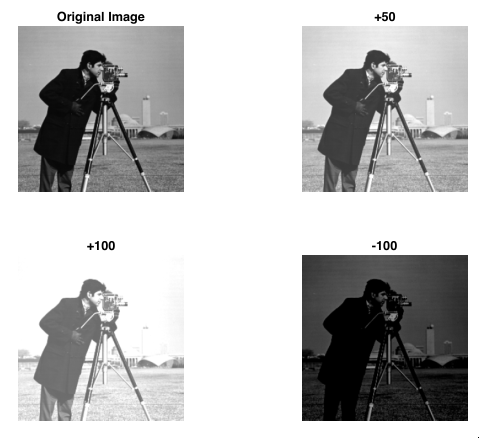
\includegraphics[width=0.7\textwidth]{arithmeticoperationsonimages.png}
\end{center}

\subsubsection{Thresholding}
\textbf{Thresholding} produces a binary image from a greyscale or colour image by setting pixels to \verb|1| or \verb|0| depending on 
whether they are above or below the threshold value.
This is useful to help separate the image foreground from the background.
Logical operators are very useful for this.

\begin{lstlisting}[language=MATLAB]
I = imread('rice.png');
T1 = I > 100;
T2 = I > 105;
T3 = I > 110;
T4 = I > 115;
T5 = I > 120;
subplot(2,3,1),imshow(I),title('Original Image');
subplot(2,3,2),imshow(T1),title('Threshold @100');
subplot(2,3,3),imshow(T2),title('Threshold @105');
subplot(2,3,4),imshow(T3),title('Threshold @110');
subplot(2,3,5),imshow(T4),title('Threshold @115');
subplot(2,3,6),imshow(T5),title('Threshold @120');
\end{lstlisting}

\section{Data Science}
\subsection{Introducing the Table in MATLAB} 
\textbf{Tables} are used to collect heterogeneous data \& metadata in a single container. 
Tables are suitable for storing column-oriented or tabular data that is often stored as columns in a text file or in a spreadsheet.
Tables can accomodate variables of different types, sizes, units, etc. 
Tables are often used to store experimental data, with rows representing the different observations and columns representing different measured variables.

Tables can be subscripted using parentheses much like ordinary numeric arrays, but in addition to numeric and logical indices, one can use a table's variable and row names (if defined) as \textbf{indices}.  
One can access individual variables in a table much like fields in a structure, using \textbf{dot subscripting}.  
One can access the contents of one or more variables using \textbf{brace subscripting}.

\bibliographystyle{unsrtnat}
\bibliography{references}
\end{document}

